\newpage
\section{Introduction}
\label{sec:introduction}

This manual describes \textit{Property-Driven Design} (PDD), a new
top-down hardware design methodology. %
It borrows ideas from so-called \textit{Test-Driven Development}
(TDD)~\cite{2002-Beck}, a software design paradigm aiming at writing high-quality code
while maintaining high productivity. %
Before we delve into PDD, let us first review TDD and discuss some
important aspects of it. 

The core idea of TDD is that before you write code for a function you
need to write the test for that function first. %
Writing tests guides the software engineer through the design
process. %
At any point during the design process, the written code is covered by
some test. Initially, the tests are very abstract, as are the
implementations of the functions. %
The functions are refined concurrently with the tests, adding more and
more behavior, until the final scope and functionality has been
reached. The flow for designing a new feature with TDD is:
\begin{enumerate}
\item Create tests that describe the desired behavior of the feature. %
\item Choose a test and implement code that fulfills the test. %
\item Check if all previously checked tests are still valid. %
\item Return to \textit{2} until all tests hold on the design. %
\end{enumerate}

The software design process is finished when all tests hold for the
design. %
This approach allows for an incremental software design process and
results in fewer design bugs, complete test coverage and a
documentation of the code. %

 \begin{wrapfigure}{l}{0.4\textwidth}
     \caption{Overview of the desired flow}
     \label{fig:PDD-overview}
     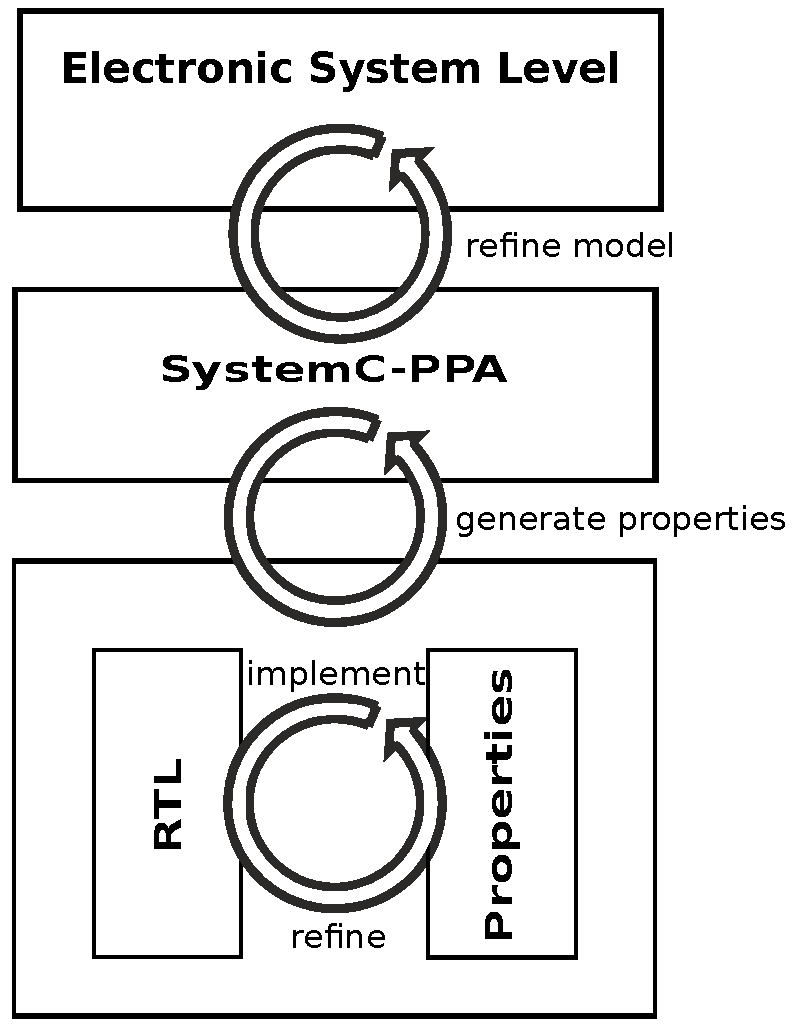
\includegraphics[width=0.4\textwidth]{fig/drawing.pdf}
 \end{wrapfigure}

%\begin{figure}
%  \begin{center}
%    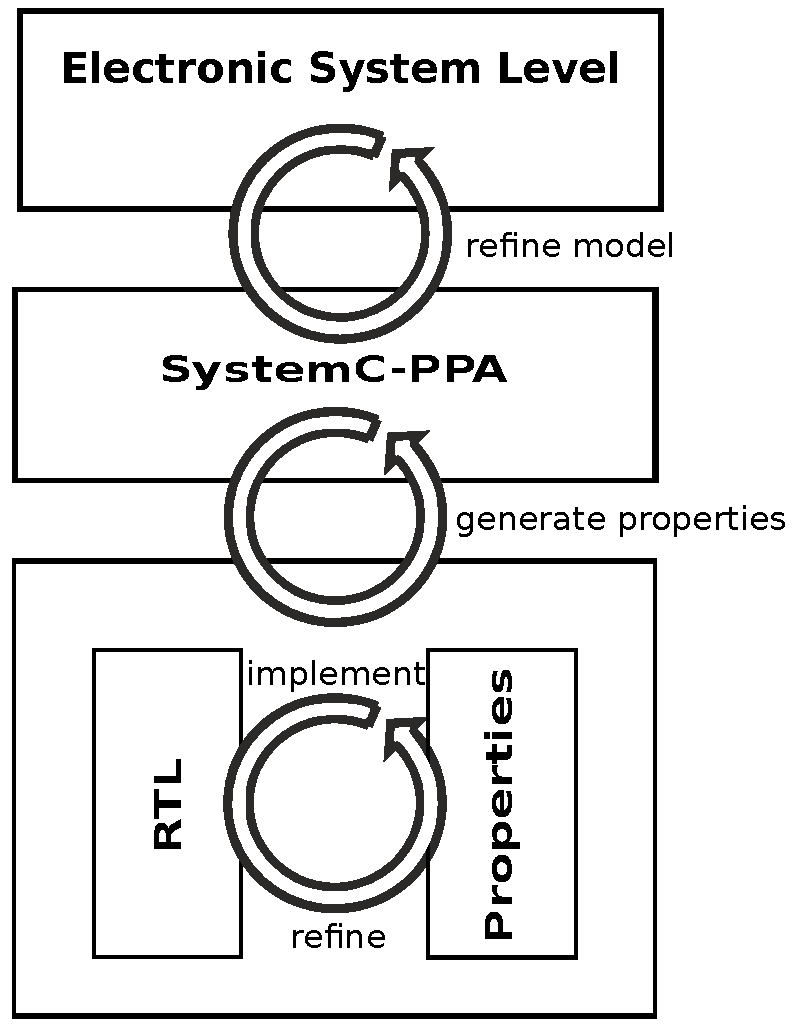
\includegraphics[width=0.3\linewidth]{fig/drawing.pdf}
%    \caption{Overview of PDD flow}
%    \label{fig:PDD-overview}
%  \end{center}
%\end{figure}

\textbf{Property-Driven Design (PDD)} takes this idea to hardware  design. %
Tests are replaced by formal properties. 
However, the designer doesn't need to write the tests. %
Instead, abstract properties are generated automatically from a high-level description. %
The PDD flow starts with a verified description of the component at the \textit{Electronic System Level} (ESL). %
  From this description the tests are generated automatically in form of interval~\cite{2014-UrdahlStoffel.etal} properties (e.g., SVA, ITL)by our tool \DeSCAM{} ("\textbf{S}ystem\textbf{C} \textbf{A}bstract \textbf{M}odel"). %
When writing RTL code, the designer only needs to refine the properties by adding information about data types and clock cycle-accurate timing. %
The general flow is similar to TDD: Properties are refined step by step. 
The designer chooses a property and implements the hardware that fulfills the property. 
Once all properties hold on the design the hardware design process is
finished. %

The design entry point of PDD is the ESL. %
Figure~\ref{fig:PDD-overview} shows an overview of the desired flow
which consists of three major steps. %
The first step is analyzing the ESL description with \DeSCAM{} and
refactoring it according to the provided feedback. %
The resulting model is now considered the golden reference for the
subsequent steps. %
The second step is the generation of abstract properties from this
model with \DeSCAM{}. %
%

Once the properties are there, the RTL design phase begins. %
Property by property is refined and VHDL code is written that
implements the behavior described by the property. %
Properties are checked, debugged and eventually proven using
commercially available property checking technology.

One novelty of PDD is that the generated properties ensure that the
RTL design has the same I/O behavior as the ESL design. %
As explained in our papers on PDD, 
the methodology ensures that the ESL description is a formally proven, sound abstraction of the RTL design. %
This allows the designer to use the ESL design as the golden model and verification results at the system level hold for the RTL without further proof. %

This has the advantage that global design decisions can be made already at the electronic system level. %
If the ESL design works correctly so will the RTL design implemented from it. %
However, also any system-level bug will appear in the RTL. %
As ESL and RTL are no longer decoupled, it is important that the ESL is thoroughly verified before PDD-based RTL implementation is
started. %

Section~\ref{sec:walk-through} will provide a step-by-step-walk-through of PDD for a simple example, followed by a more detailed explanation of PDD in the subsequent sections. %
The \textit{installation} of the software tool \DeSCAM{} is explained in Section~\ref{sec:installation}. %
All example files are available on our GitHub page~\cite{web-DeSCAM}. %

%%% Local Variables: 
%%% mode: latex
%%% TeX-master: "binder"
%%% End: 

